\documentclass{exam}

\usepackage{units} 
\usepackage{graphicx}
\usepackage[fleqn]{amsmath}
\usepackage{cancel}
\usepackage{float}
\usepackage{mdwlist}
\usepackage{booktabs}
\usepackage{cancel}
\usepackage{polynom}
\usepackage{caption}
\usepackage{fullpage}
\usepackage{xfrac}
\usepackage{enumerate}

\newcommand{\degree}{\ensuremath{^\circ}} 
\everymath{\displaystyle}

\usepackage{2in1, lscape} 

\title{Math 142 Notes \\ Section 5.3}

\date{September 11, 2013}

\begin{document}

  \maketitle
  \tableofcontents

  \section{Sine/Cosine Applications}

  \subsection{Spring and Weight}
  \[
    x = \cos \left[ \sqrt{\sfrac{k}{m}} t \right]
  \]
  \begin{itemize}
    \item force proportional to position: $f = kx$
    \item when $x$ is close to $\pm 1$, velocity is close to $0$
    \item velocity is sine graph
  \end{itemize}

  \subsection{Pendulum}
  \[
    x = \cos kt 
  \]
  \begin{itemize}
    \item force proportional to position: $f = kx$
    \item when $x$ is close to $\pm 1$, velocity is close to $0$
    \item velocity is sine graph
  \end{itemize}

  \subsection{Wheel Turning}
  Starting from point on x-axis:
  \begin{align*}
    x &= \cos kt \\
    y &= \sin kt \\
  \end{align*}

  \begin{itemize}
    \item visualize with shadows
    \item when $x$ is close to $\pm 1$, $y$ changes rapidly and vice-versa
  \end{itemize}

  \section{Basic Graph}
  \begin{itemize*}
    \item draw single period of sine using known points
    \item draw single period of cosine using known points
  \end{itemize*}

  \begin{itemize*}
    \item sine, cosine, etc., repeat as you go around the unit circle again
    \item $\sin(t \pm 2n \pi) = \sin t$ for any integer $n$, etc.
    \item a function is periodic if there is some $p$ where $f(t + p) = f(t)$ for any value of $t$.  The smallest
      $p$ that works is the {\em period} of $f$.
    \item to graph a periodic function, you only need one period
    \item The period of sine and cosine is $2 \pi$.  
  \end{itemize*}

  \section{Amplitude}
  \subsection{Description}
  \[
    y = a \sin x
  \]

  \begin{itemize*}
    \item $|a|$ is the amplitude
    \item determines vertical scale
  \end{itemize*}

  \subsection{Examples}
  \begin{enumerate}
    \item $y = 2 \sin x$
    \item $y = \sfrac{1}{2} \sin x$
    \item $y = -3 \cos x$
  \end{enumerate}

  \section{Period}
  \[
    y = \sin kx
  \]

  \subsection{Shorter Period}
  \[
    y = \sin 2x
  \]

  \begin{tabular}[H]{lrr}
    \toprule
    $x$                & $2x$               & $\sin 2x$ \\
    \midrule
    $0$                & $0$                & $0$ \\
    $\sfrac{\pi}{4}$   & $\sfrac{\pi}{2}$   & $1$ \\
    $\sfrac{\pi}{2}$   & $\pi$              & $0$ \\
    $\sfrac{3 \pi}{4}$ & $\sfrac{3 \pi}{2}$ & $-1$ \\
    $\pi$              & $2 \pi$            & $0$ \\
    \bottomrule
  \end{tabular}

  Cycle repeats every $\pi$

  \subsection{Longer Period}
  \[
    y = \sin \frac{1}{2} x
  \]

  \begin{tabular}[H]{lrr}
    \toprule
    $x$     & $\sfrac{x}{2}$     & $\sin \sfrac{x}{2}$ \\
    \midrule
    $0$     & $0$                & $0$ \\
    $\pi$   & $\sfrac{\pi}{2}$   & $1$ \\
    $2 \pi$ & $\pi$              & $0$ \\
    $3\pi$  & $\sfrac{3 \pi}{2}$ & $-1$ \\
    $4 \pi$ & $2 \pi$            & $0$ \\
    \bottomrule
  \end{tabular}

  Cycle repeats every $4 \pi$

  \subsection{General}
  \begin{align*}
    \sin(kx) & = \sin(kx + 2 \pi n) \\
    \sin(kx) & = \sin(kx + 2 \pi n) \\
             & = \sin \left[ k \left(x + \frac{2 \pi}{k} n \right) \right ] \\
  \end{align*}

  \begin{itemize*}
    \item $\sfrac{2 \pi}{k}$ is the period
    \item determines horizontal scale
    \item bigger $k$ means travel faster around the unit circle and a shorter period
    \item bigger $k$ means compressed horizontally
    \item $k = 1$ gives a period of $2 \pi$
  \end{itemize*}

  \subsection{Examples}
  \begin{enumerate*}
    \item $y = \sin 3x$; $p = \sfrac{2 \pi}{3}$
    \item $y = \sin \frac{3}{2} x$; $p = \sfrac{4 \pi}{3}$
  \end{enumerate*}

  \section{General Graph}
  \subsection{General Form}
  \[
    y = a \sin k(x - b)
  \]

  \begin{itemize*}
    \item $|a|$ is the amplitude---determines how big the peaks and valleys are
    \item $\sfrac{2 \pi}{k}$ is the period---determines the horizontal compression
    \item $b$ is the phase shift---determines the horizontal shift
    \item to graph one period, graph from $b$ to $b + \sfrac{2 \pi}{k}$
  \end{itemize*}

  \section{Examples}

  \begin{description}
    \item[1]
      \begin{figure}[H]
        \centering
        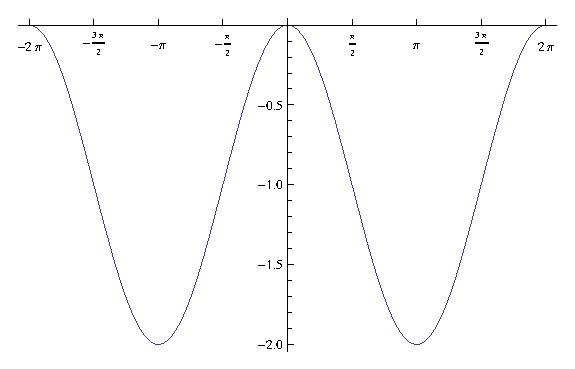
\includegraphics[scale=0.8]{example01.eps}

        $f(x) = -1 + \cos x$
      \end{figure}

    \item[2]
      \begin{figure}[H]
        \centering
        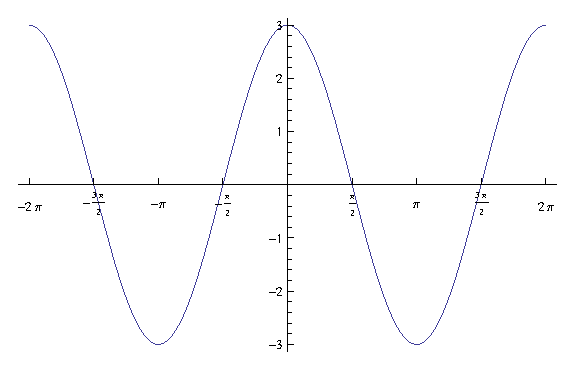
\includegraphics[scale=0.8]{example02.eps}

        $g(x) = 3 \cos x$
      \end{figure}

    \item[3]
      \begin{figure}[H]
        \centering
        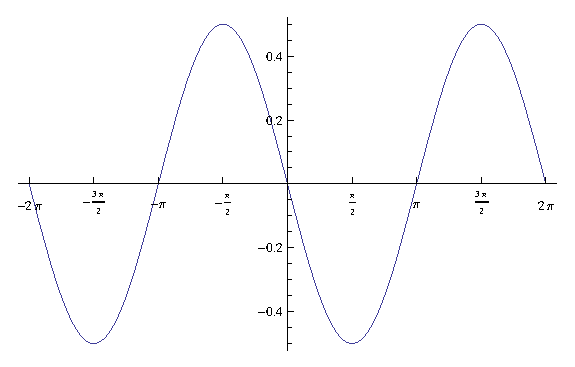
\includegraphics[scale=0.9]{example03.eps}

        $g(x) = - \sfrac{1}{2} \sin x$
      \end{figure}

    \item[4]
      \begin{figure}[H]
        \centering
        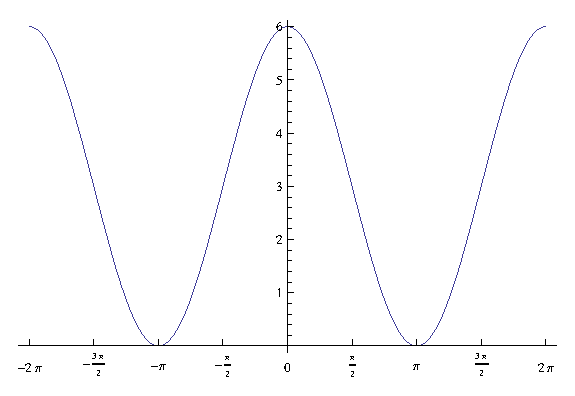
\includegraphics[scale=0.9]{example04.eps}

        $g(x) = 3 + 3 \cos x$
      \end{figure}

    \item[5]
      \begin{figure}[H]
        \centering
        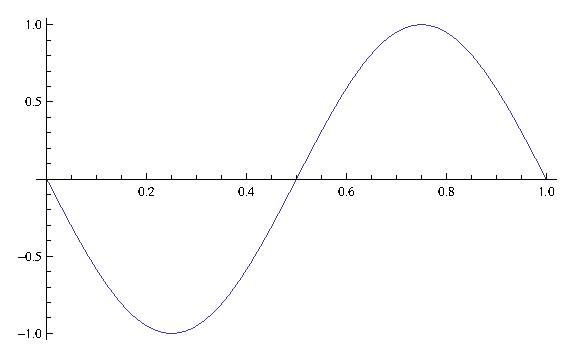
\includegraphics[scale=0.9]{example05.eps}

        $y = - \sin 2 \pi x$
      \end{figure}

      \begin{tabular}[H]{lr}
        \toprule
        amplitude & $-1$ \\
        period    & $1$ \\
        phase     & $0$ \\
        \bottomrule
      \end{tabular}

      \item[6]
        \begin{figure}[H]
          \centering
          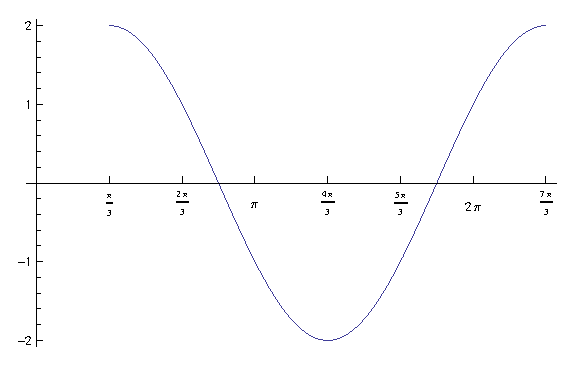
\includegraphics[scale=0.8]{example06.eps}

          $y = 2 \cos \left( x - \frac{\pi}{3} \right)$
        \end{figure}

        \begin{tabular}[H]{lr}
          \toprule
          amplitude   & $2$ \\
          period      & $2 \pi$ \\
          phase shift & $\sfrac{\pi}{3}$ \\
          \bottomrule
        \end{tabular}

      \item[7]
        \begin{figure}[H]
          \centering
          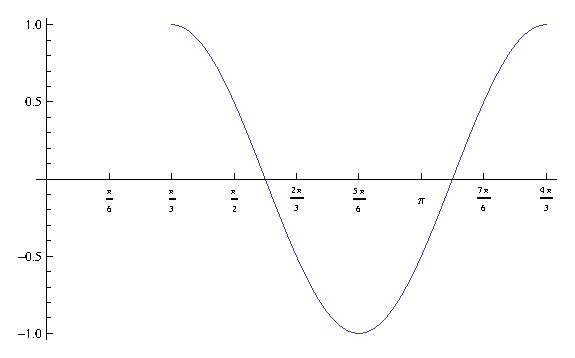
\includegraphics[scale=0.8]{example07.eps}

          $y = \cos \left[ 2 \left( x - \frac{\pi}{3} \right) \right]$
        \end{figure}

        \begin{tabular}[H]{lr}
          \toprule
          amplitude   & $1$ \\
          period      & $\pi$ \\
          phase shift & $\sfrac{\pi}{3}$ \\
          \bottomrule
        \end{tabular}

      \item[8]
        \begin{figure}[H]
          \centering
          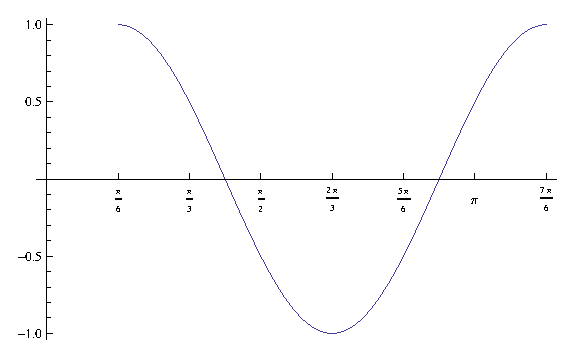
\includegraphics[scale=0.8]{example08.eps}

          $y = \cos \left( 2x - \frac{\pi}{3} \right) = \cos \left[ 2 \left( x - \frac{\pi}{6} \right) \right]$
        \end{figure}

        \begin{tabular}[H]{lr}
          \toprule
          amplitude   & $1$ \\
          period      & $\pi$ \\
          phase shift & $\sfrac{\pi}{6}$ \\
          \bottomrule
        \end{tabular}

      \item[9]
        \begin{figure}[H]
          \centering
          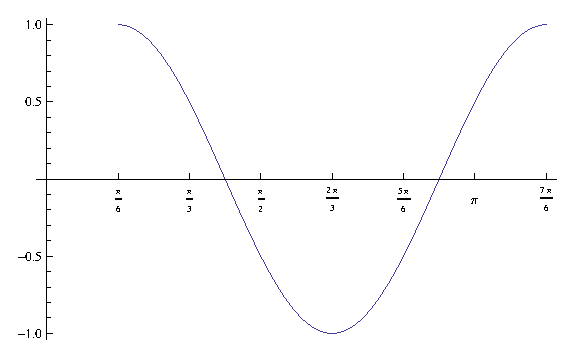
\includegraphics[scale=0.8]{example09.eps}

          $y = \cos \left( 2x - \frac{\pi}{3} \right) = \cos \left[ 2 \left( x - \frac{\pi}{6} \right) \right]$
        \end{figure}

        \begin{tabular}[H]{lr}
          \toprule
          amplitude   & $1$ \\
          period      & $\pi$ \\
          phase shift & $\sfrac{\pi}{6}$ \\
          \bottomrule
        \end{tabular}

      \item[10]
        \begin{figure}[H]
          \centering
          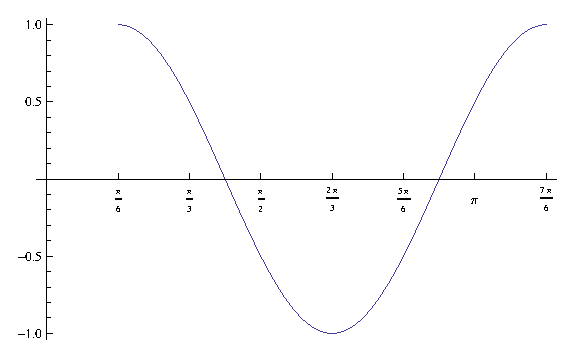
\includegraphics[scale=0.9]{example08.eps}

          $y = \sin \left( 2 \pi x + \pi \right) = \sin \left[ 2 \pi \left( x + \frac{1}{2} \right) \right]$
        \end{figure}

        \begin{tabular}[H]{lr}
          \toprule
          amplitude   & $1$ \\
          period      & $\pi$ \\
          phase shift & $\sfrac{\pi}{6}$ \\
          \bottomrule
        \end{tabular}

  \end{description}

\end{document}
